\section{Statistical Tests}
\label{sec:appendix_statistics}


\subsection{F-Tests}
\label{sec:appendix_ftests}



Figures~\ref{fig:ftest16}~to~\ref{fig:ftest18} show the plots of these F-tests used to determine the optimal Transfer Function.

            \begin{figure}[!htbp]
                \begin{center}
                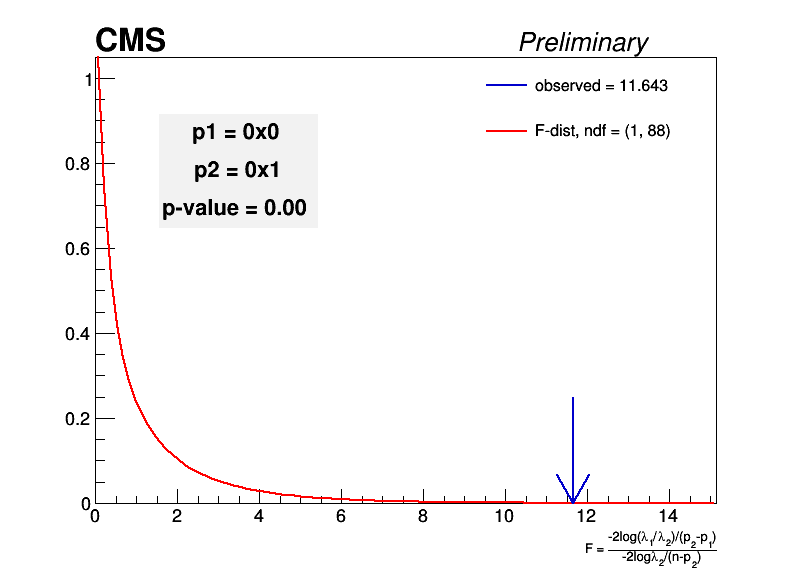
\includegraphics[width=0.4\linewidth]{Plots/tests/ftest_cen_0x0_vs_0x1_2016.png}
                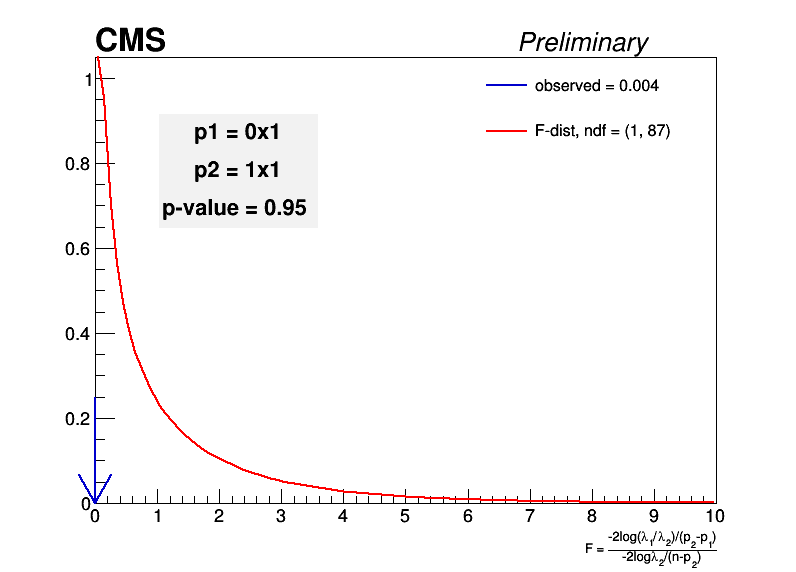
\includegraphics[width=0.4\linewidth]{Plots/tests/ftest_cen_0x1_vs_1x1_2016.png}
                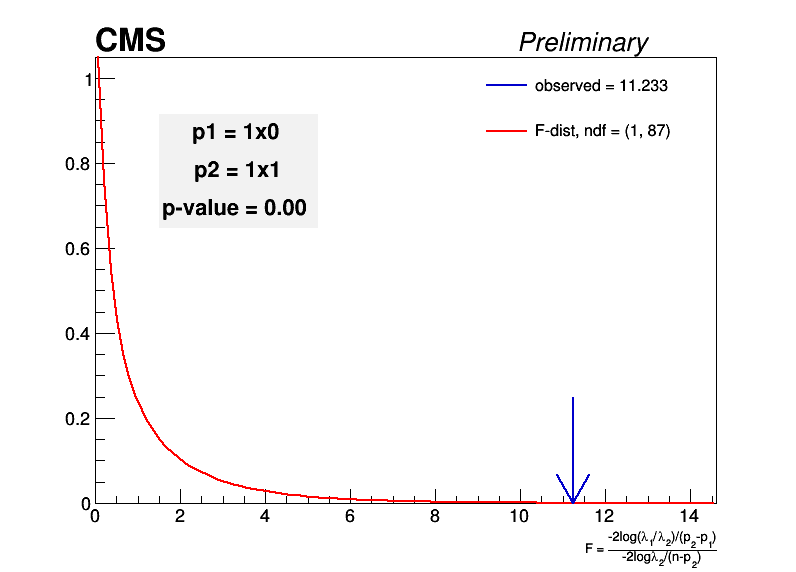
\includegraphics[width=0.4\linewidth]{Plots/tests/ftest_cen_1x0_vs_1x1_2016.png}
                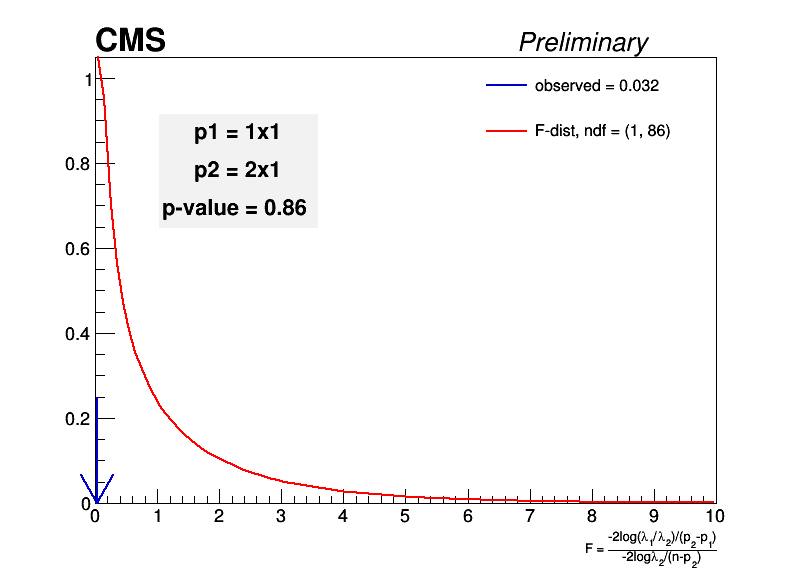
\includegraphics[width=0.4\linewidth]{Plots/tests/ftest_cen_1x1_vs_2x1_2016.png}
    
                    \caption{F-test for 2016 central background estimate, comparing the 0x1 TF to the 0x0 TF (top left), 1x1 TF to the 0x1 TF (top right), 1x1 TF to the 1x0 TF (bottom left), and 2x1 TF to the 2x1 TF (bottom right).}
                    \label{fig:ftest16}
                \end{center}
            \end{figure}
            


            \begin{figure}[!htbp]
                \begin{center}
                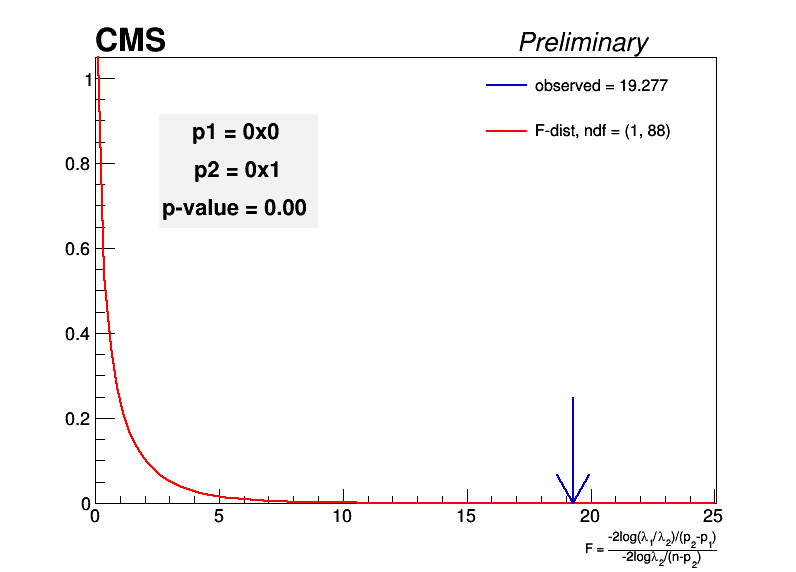
\includegraphics[width=0.4\linewidth]{Plots/tests/ftest_cen_0x0_vs_0x1_2017.png}
                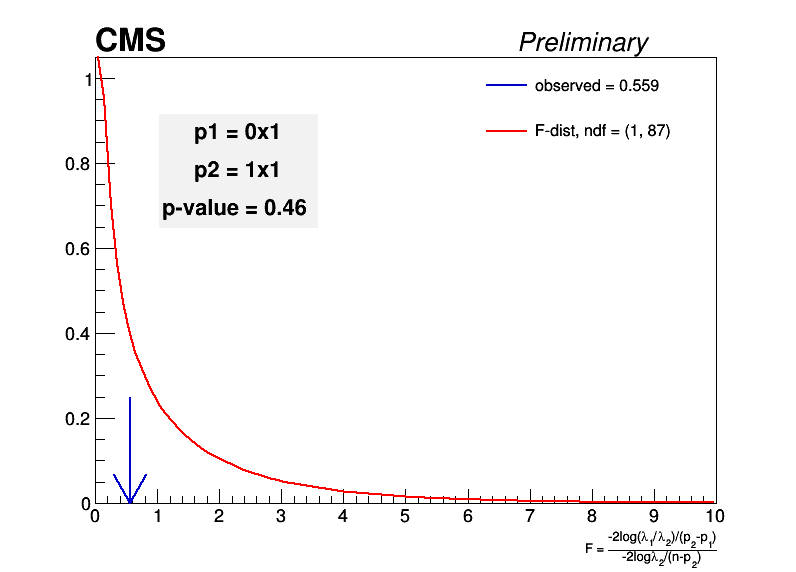
\includegraphics[width=0.4\linewidth]{Plots/tests/ftest_cen_0x1_vs_1x1_2017.png}
                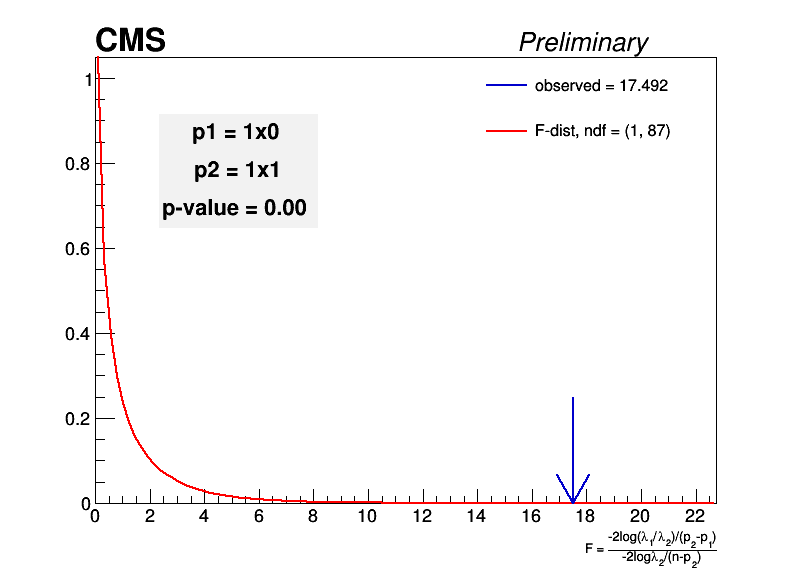
\includegraphics[width=0.4\linewidth]{Plots/tests/ftest_cen_1x0_vs_1x1_2017.png}
                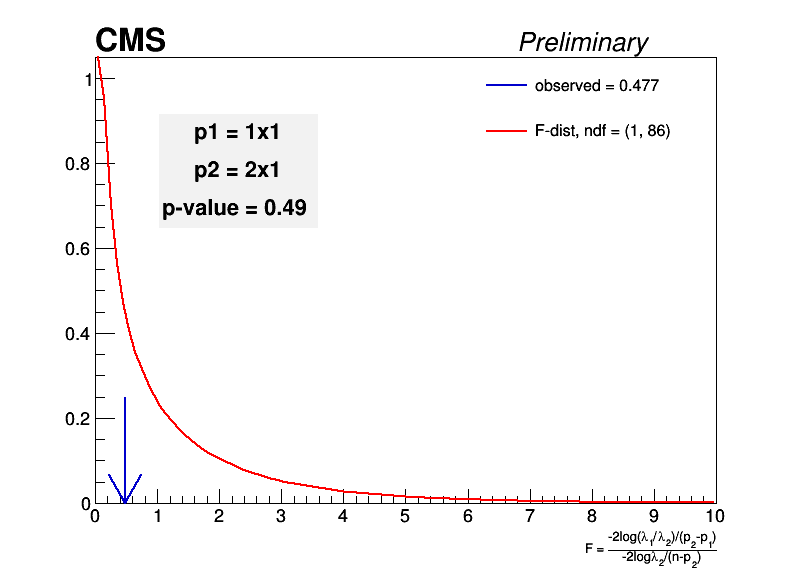
\includegraphics[width=0.4\linewidth]{Plots/tests/ftest_cen_1x1_vs_2x1_2017.png}
    
                    \caption{F-test for 2017 central background estimate, comparing the 0x1 TF to the 0x0 TF (top left), 1x1 TF to the 0x1 TF (top right), 1x1 TF to the 1x0 TF (bottom left), and 2x1 TF to the 2x1 TF (bottom right).}
                    \label{fig:ftest17}
                \end{center}
            \end{figure}
            

            \begin{figure}[!htbp]
                \begin{center}
                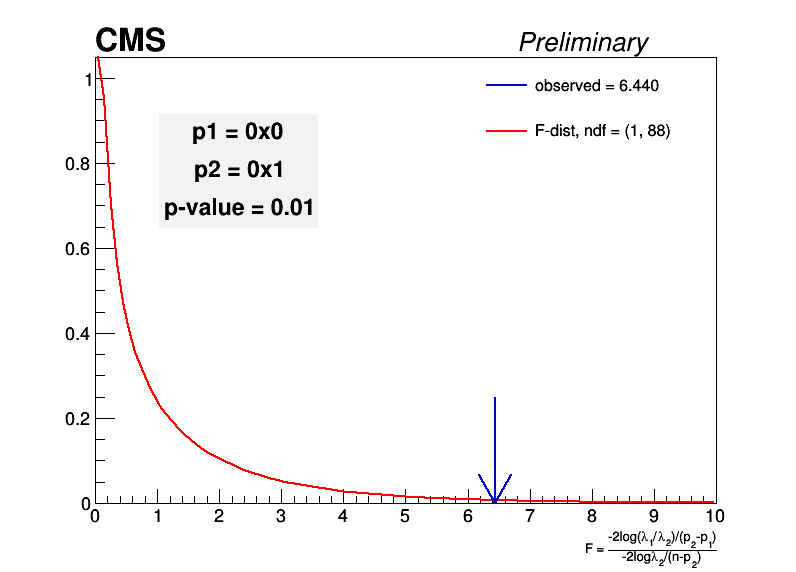
\includegraphics[width=0.4\linewidth]{Plots/tests/ftest_cen_0x0_vs_0x1_2018.png}
                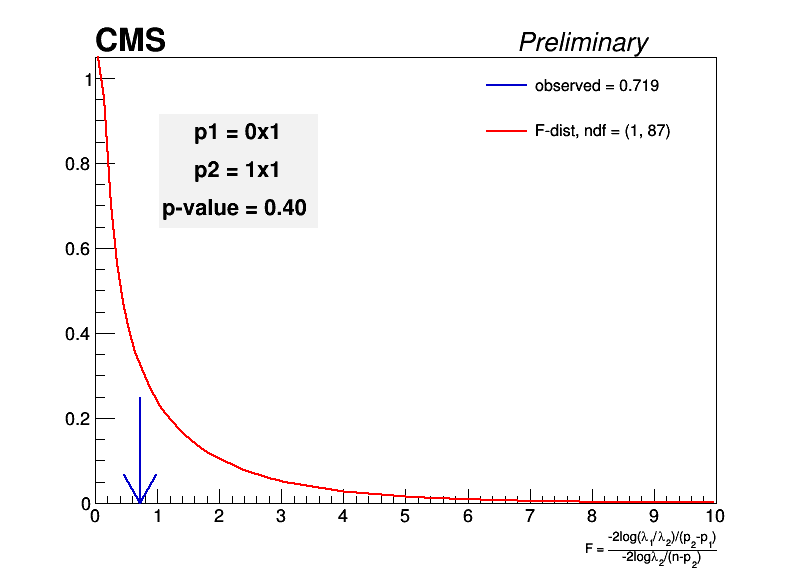
\includegraphics[width=0.4\linewidth]{Plots/tests/ftest_cen_0x1_vs_1x1_2018.png}
                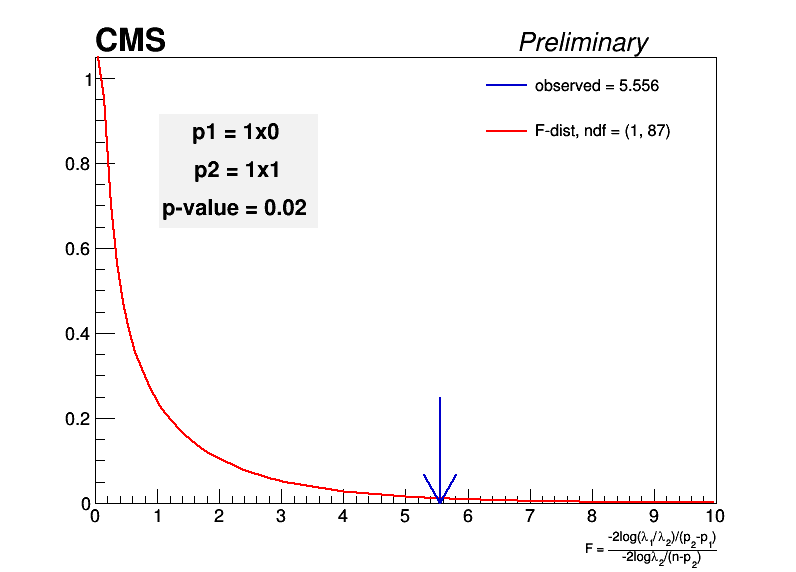
\includegraphics[width=0.4\linewidth]{Plots/tests/ftest_cen_1x0_vs_1x1_2018.png}
                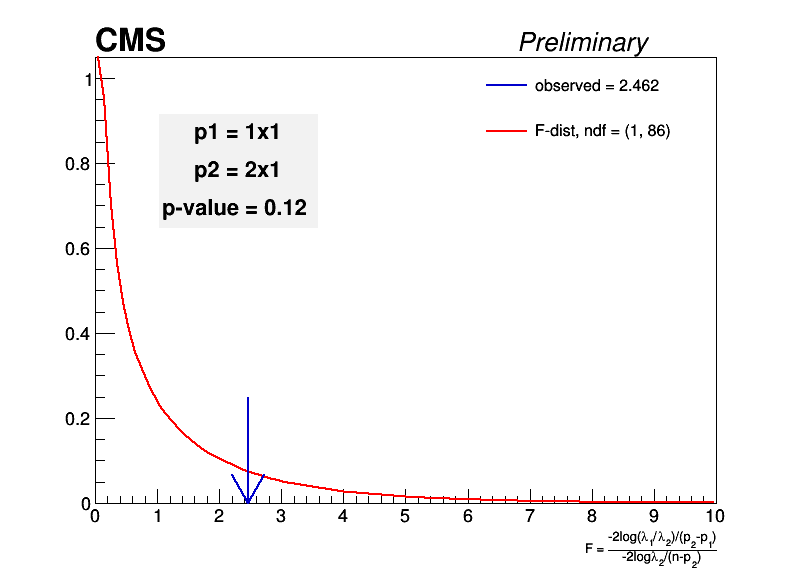
\includegraphics[width=0.4\linewidth]{Plots/tests/ftest_cen_1x1_vs_2x1_2018.png}
    
                    \caption{F-test for 2018 central background estimate, comparing the 0x1 TF to the 0x0 TF (top left), 1x1 TF to the 0x1 TF (top right), 1x1 TF to the 1x0 TF (bottom left), and 2x1 TF to the 2x1 TF (bottom right).}
                    \label{fig:ftest18}
                \end{center}
            \end{figure}
            
            
                        \begin{figure}[!htbp]
                \begin{center}
                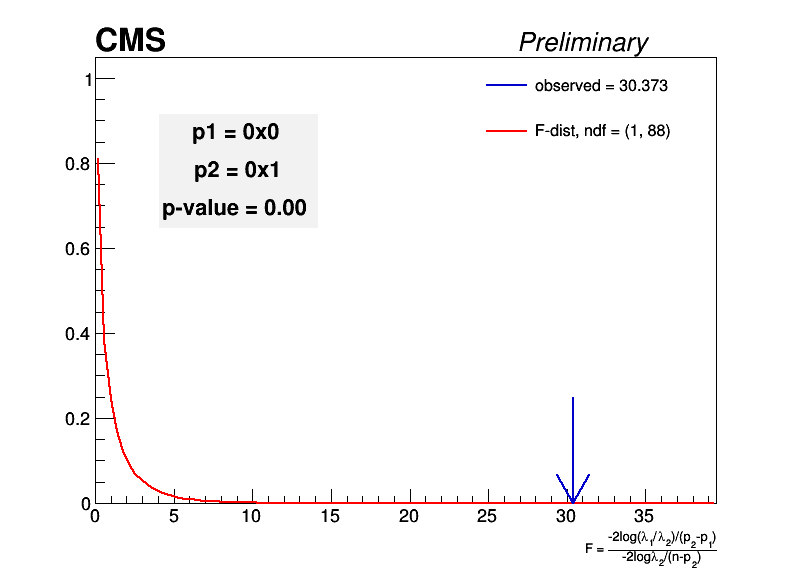
\includegraphics[width=0.4\linewidth]{Plots/tests/ftest_fwd_0x0_vs_0x1_2016.png}
                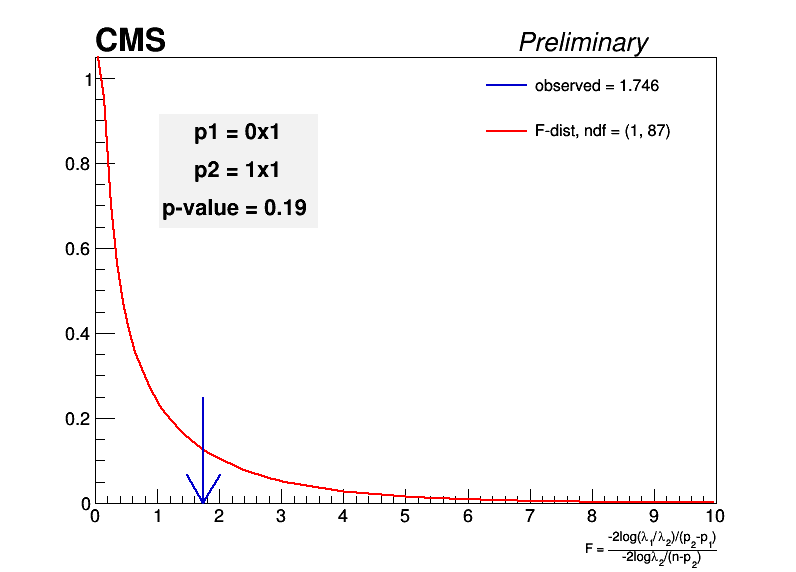
\includegraphics[width=0.4\linewidth]{Plots/tests/ftest_fwd_0x1_vs_1x1_2016.png}
                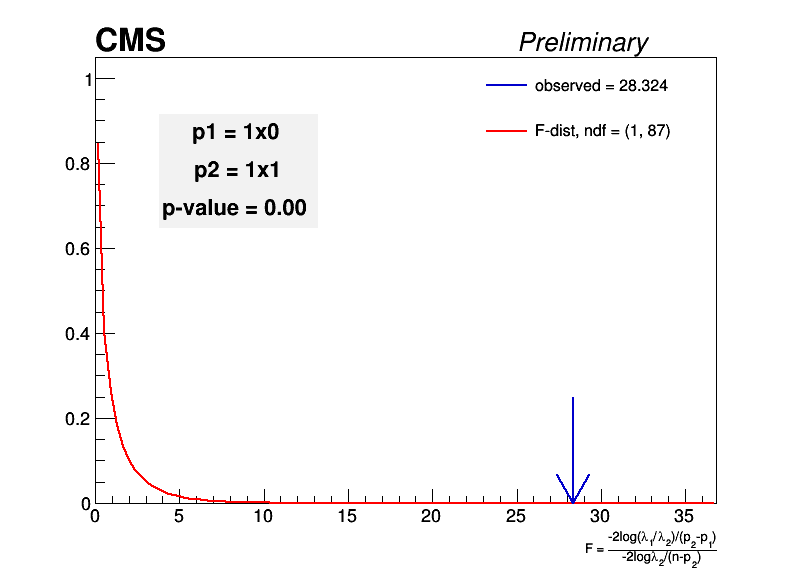
\includegraphics[width=0.4\linewidth]{Plots/tests/ftest_fwd_1x0_vs_1x1_2016.png}
                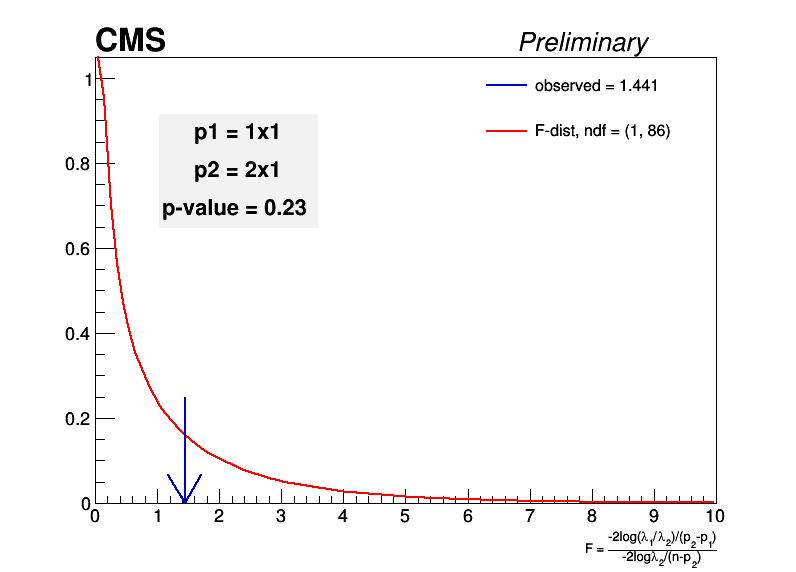
\includegraphics[width=0.4\linewidth]{Plots/tests/ftest_fwd_1x1_vs_2x1_2016.png}
    
                    \caption{F-test for 2016 forward background estimate, comparing the 0x1 TF to the 0x0 TF (top left), 1x1 TF to the 0x1 TF (top right), 1x1 TF to the 1x0 TF (bottom left), and 2x1 TF to the 2x1 TF (bottom right).}
                    \label{fig:ftest16}
                \end{center}
            \end{figure}
            


            \begin{figure}[!htbp]
                \begin{center}
                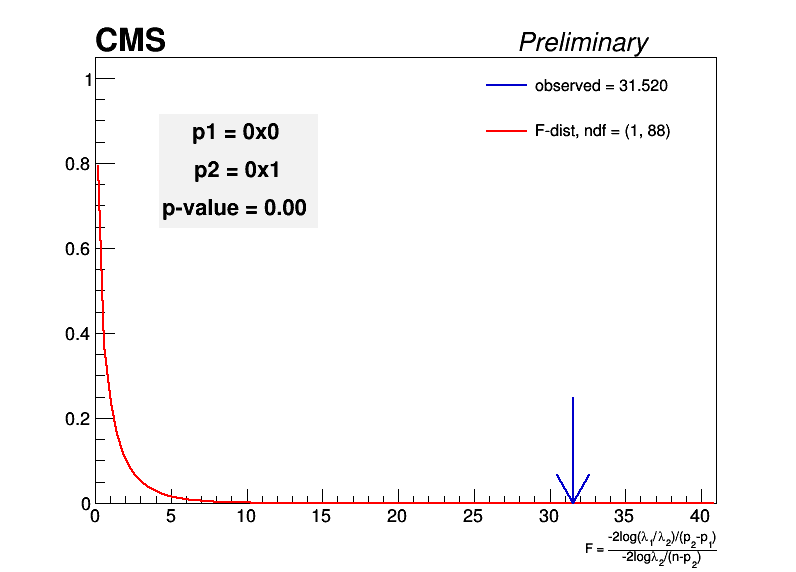
\includegraphics[width=0.4\linewidth]{Plots/tests/ftest_fwd_0x0_vs_0x1_2017.png}
                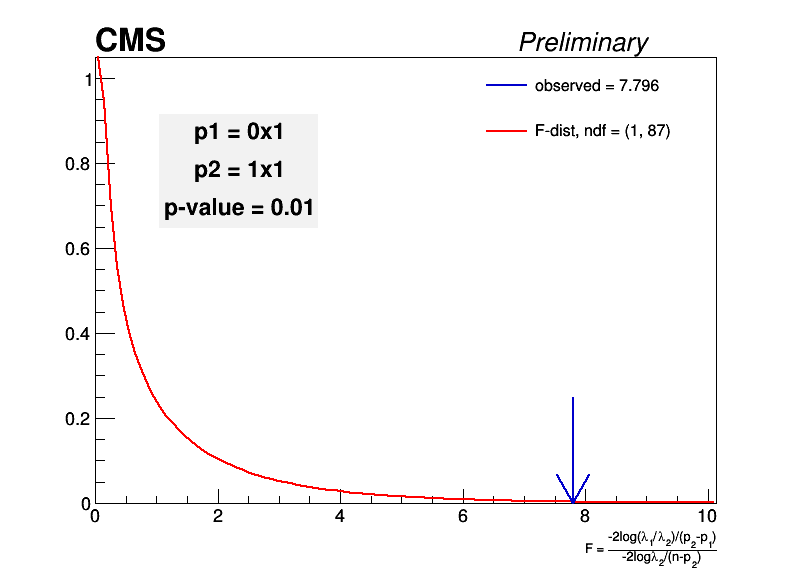
\includegraphics[width=0.4\linewidth]{Plots/tests/ftest_fwd_0x1_vs_1x1_2017.png}
                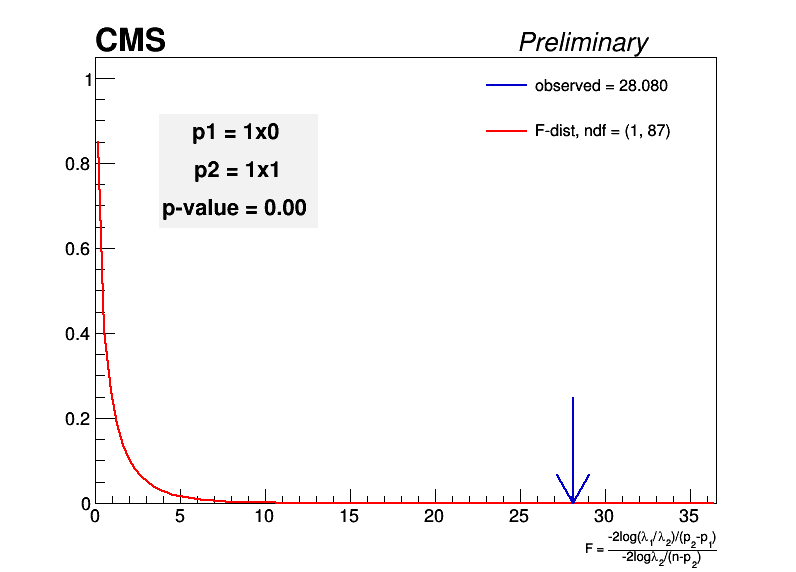
\includegraphics[width=0.4\linewidth]{Plots/tests/ftest_fwd_1x0_vs_1x1_2017.png}
                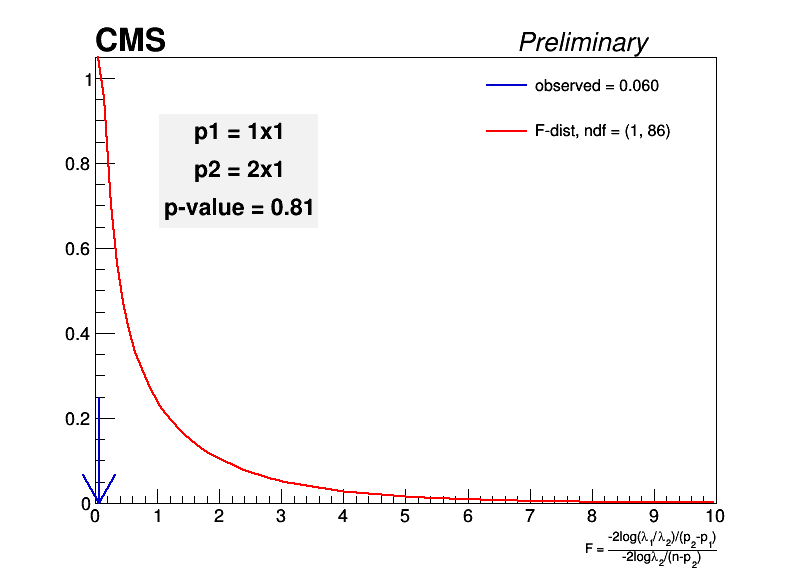
\includegraphics[width=0.4\linewidth]{Plots/tests/ftest_fwd_1x1_vs_2x1_2017.png}
    
                    \caption{F-test for 2017 forward background estimate, comparing the 0x1 TF to the 0x0 TF (top left), 1x1 TF to the 0x1 TF (top right), 1x1 TF to the 1x0 TF (bottom left), and 2x1 TF to the 2x1 TF (bottom right).}
                    \label{fig:ftest17}
                \end{center}
            \end{figure}
            

            \begin{figure}[!htbp]
                \begin{center}
                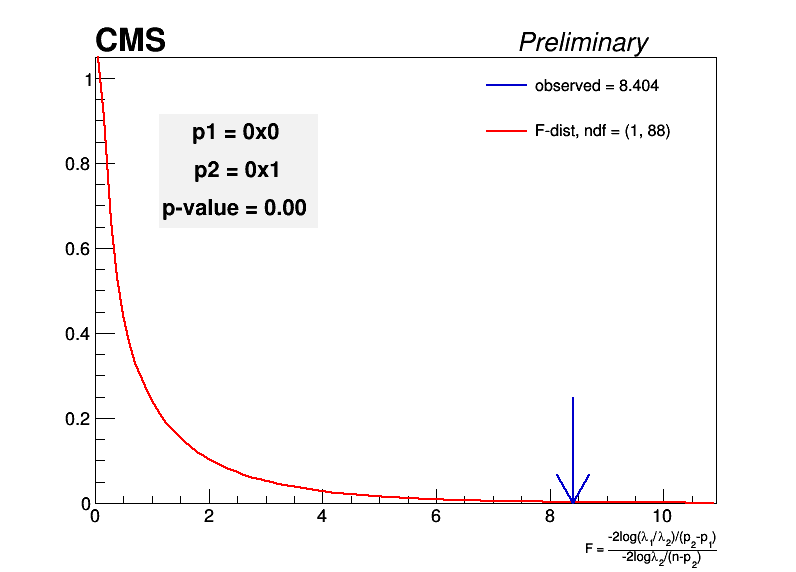
\includegraphics[width=0.4\linewidth]{Plots/tests/ftest_fwd_0x0_vs_0x1_2018.png}
                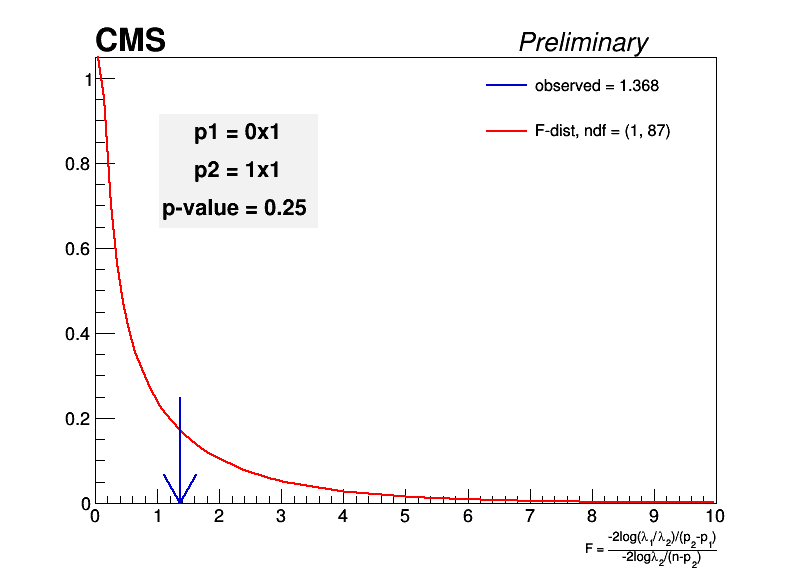
\includegraphics[width=0.4\linewidth]{Plots/tests/ftest_fwd_0x1_vs_1x1_2018.png}
                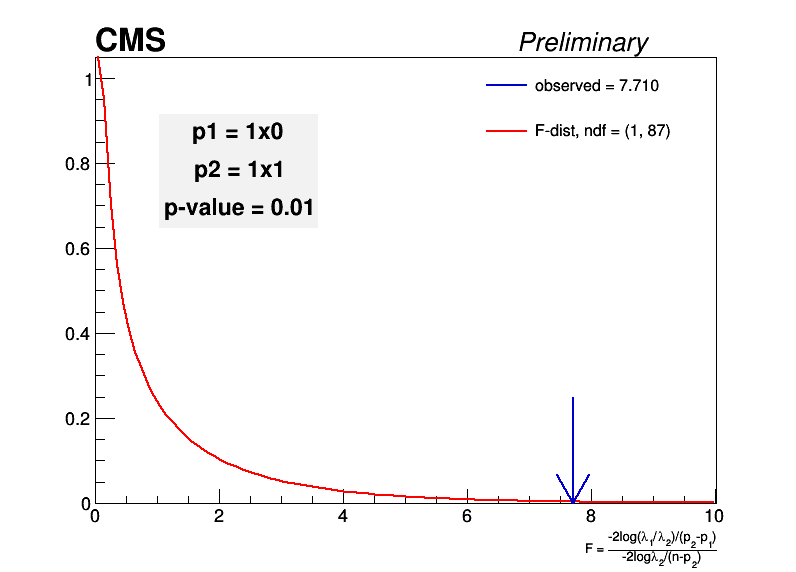
\includegraphics[width=0.4\linewidth]{Plots/tests/ftest_fwd_1x0_vs_1x1_2018.png}
                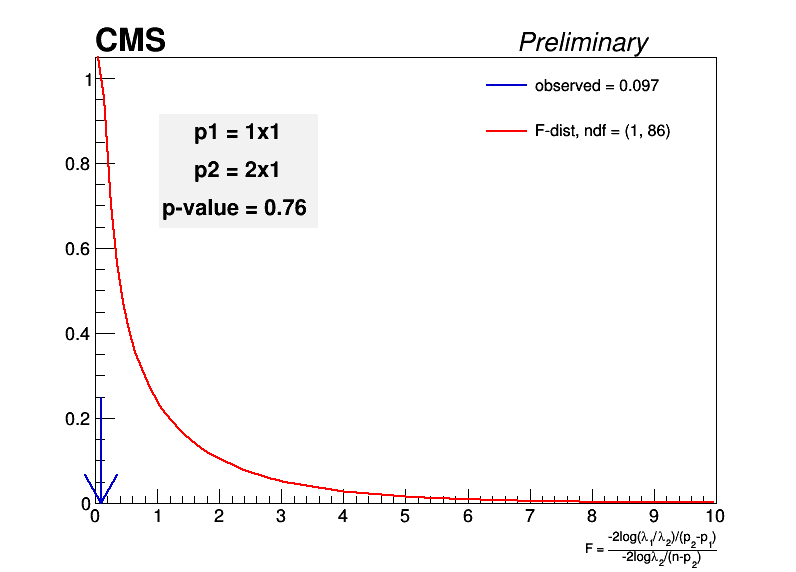
\includegraphics[width=0.4\linewidth]{Plots/tests/ftest_fwd_1x1_vs_2x1_2018.png}
    
                    \caption{F-test for 2018 forward background estimate, comparing the 0x1 TF to the 0x0 TF (top left), 1x1 TF to the 0x1 TF (top right), 1x1 TF to the 1x0 TF (bottom left), and 2x1 TF to the 2x1 TF (bottom right).}
                    \label{fig:ftest18}
                \end{center}
            \end{figure}
   
   
   
   
\subsection{Goodness of Fit}
\label{sec:appendix_gof}


The Goodness of Fit tests run separately for each year and rapidity region are plotted in Figure~\ref{fig:gof}.

         
\begin{figure}[!htbp]
                \begin{center}
                 \includegraphics[width=0.45\linewidth]{Plots/tests/gof_plot_cen16.pdf}
		\includegraphics[width=0.45\linewidth]{Plots/tests/gof_plot_fwd16.pdf} \\
                 \includegraphics[width=0.45\linewidth]{Plots/tests/gof_plot_cen17.pdf} 
                 \includegraphics[width=0.45\linewidth]{Plots/tests/gof_plot_fwd17.pdf} \\
		\includegraphics[width=0.45\linewidth]{Plots/tests/gof_plot_cen18.pdf}
                 \includegraphics[width=0.45\linewidth]{Plots/tests/gof_plot_fwd18.pdf}

                    \caption{Goodness of Fit test for 2016 (top), 2017 (middle), 2018 (bottom) central (left) and forward (right) regions.}
                    \label{fig:gof}
                \end{center}
            \end{figure}
